%# -*- coding: utf-8-unix -*-
% !TEX program = xelatex
% !TEX root = ../thesis.tex
% !TEX encoding = UTF-8 Unicode
%%==================================================
%% chapter02.tex for SJTU Master Thesis
%% based on CASthesis
%% modified by wei.jianwen@gmail.com
%% Encoding: UTF-8
%%==================================================

\chapter{Competition with different updating rules}
\label{chap4}
In this chapter, we would control dynamics orders between layers and updating rules of nodes and edges. With changing these updating rules, it would be investigated how the states of network are changed. Here, each layer consists of \textit{Barabasi-Albert(BA)} network that has $N$ nodes with attaching new nodes each with $K$ edges that are preferentially attached to existing nodes with high degree as introduced in \parencite{barabasi1999}. Each node of one layer is connected with a random node on the other layer. This means each node has only $1$ external edge. Simulations are performed on network with $N=2048$, and $K=3$.

When considering updating rules on two-layer networks, there are many ways to update the state of nodes. Dynamics orders of two-layers can be considered whether layer A works first or layer B works first or both layers work together. And, orders of nodes can be thought as whether the states of nodes are changed simultaneously or sequentially or randomly. Orders of edges connected with a node also can be deliberated as whether edges are activated on a node sequentially or simultaneously or randomly. However, in layer B dynamics, order of edges in one node always follows the simultaneous updating rule, because dynamics formula already considers the states of all connected neighbor nodes simultaneously. To sum up, as shown in Table.\ref{25updating_rules}, 25 updating rules would be considered according to layers, nodes and edges. \\

\begin{table}[htp]
	\scriptsize
	\begin{center}
		\begin{tabular}{c|c|c|c|c}
			Order of layers                                  & \multicolumn{2}{|c|}{Layer A}                                      & Layer B                & remarks   \\ \cline{2-4}
			& Order of nodes                 & Order of edges                     & Order of nodes         &  \\ \hline
			\multirow{10}{*}{Layer A $\rightarrow$ Layer B} & \multirow{4}{*}{Sequential}    & \multirow{2}{*}{Sequential}        & Sequential             & O(o, o) $\to$ D(o) \\  \cline{4-5}  
			&                                &                                    & Simultaneous           & O(o, o) $\to$ D(s) \\  \cline{3-5}     
			&                                & \multirow{2}{*}{Simultaneous}      & Sequential             & O(o, s) $\to$ D(o) \\  \cline{4-5} 
			&                                &                                    & Simultaneous           & O(o, s) $\to$ D(s) \\  \cline{2-5} 
			& \multirow{4}{*}{Simultaneous}  & \multirow{2}{*}{Sequential}        & Sequential             & O(s, o) $\to$ D(o) \\  \cline{4-5}
			&                                &                                    & Simultaneous           & O(s, o) $\to$ D(s) \\  \cline{3-5}
			&                                & \multirow{2}{*}{Simultaneous}      & Sequential             & O(s, s) $\to$ D(o) \\  \cline{4-5}
			&                                &                                    & Simultaneous           & O(s, s) $\to$ D(s) \\  \cline{2-5}
			& \multirow{2}{*}{Random}        & \multirow{2}{*}{Random}            & Sequential             & O(r, r) $\to$ D(o) \\  \cline{4-5}
			&                                &                                    & Simultaneous           & O(r, r) $\to$ D(s) \\   \hline
			\multirow{10}{*}{Layer A $\leftarrow$ Layer B}  & \multirow{4}{*}{Sequential}    & \multirow{2}{*}{Sequential}        & Sequential             & O(o, o) $\leftarrow$ D(o) \\  \cline{4-5}  
			&                                &                                    & Simultaneous           & O(o, o) $\leftarrow$ D(s) \\  \cline{3-5}     
			&                                & \multirow{2}{*}{Simultaneous}      & Sequential             & O(o, s) $\leftarrow$ D(o) \\  \cline{4-5} 
			&                                &                                    & Simultaneous           & O(o, s) $\leftarrow$ D(s) \\  \cline{2-5} 
			& \multirow{4}{*}{Simultaneous}  & \multirow{2}{*}{Sequential}        & Sequential             & O(s, o) $\leftarrow$ D(o) \\  \cline{4-5}
			&                                &                                    & Simultaneous           & O(s, o) $\leftarrow$ D(s) \\  \cline{3-5}
			&                                & \multirow{2}{*}{Simultaneous}      & Sequential             & O(s, s) $\leftarrow$ D(o) \\  \cline{4-5}
			&                                &                                    & Simultaneous           & O(s, s) $\leftarrow$ D(s) \\  \cline{2-5}
			& \multirow{2}{*}{Random}        & \multirow{2}{*}{Random}            & Sequential             & O(r, r) $\leftarrow$ D(o) \\  \cline{4-5}
			&                                &                                    & Simultaneous           & O(r, r) $\leftarrow$ D(s) \\   \hline
			\multirow{2}{*}{Layer A $\leftrightarrow$ Layer B}& \multirow{2}{*}{Simultaneous}& Sequential                         & Simultaneous           & O(s, o) $\leftrightarrow$ D(s) \\ \cline{3-5}
			&                                & Simultaneous                       & Simultaneous           & O(s, s) $\leftrightarrow$ D(s) \\ \hline
			\multirow{3}{*}{Layer A $\Leftrightarrow$ Layer B}& \multirow{2}{*}{Sequential}  & Sequential                         & Sequential             & O(o, o) $\Leftrightarrow$ D(o) \\ \cline{3-5}
			&                                & Simultaneous                       & Sequential             & O(o, s) $\Leftrightarrow$ D(o) \\ \cline{2-5}
			& Random                         & Random                             & Random                 & O(r, r) $\Leftrightarrow$ D(r) \\ \hline
			
		\end{tabular}
	\end{center}
	\caption{25 updating rules according to order of layers, nodes, and edges}
	\label{25updating_rules}
\end{table}

Updating rules are indicated as follows. `O' and `D'  represent `Opinion layer' and `Decision Making layer' individually. `o' and `s' indicate sequential updating rule and simultaneous updating rule individually. And the arrow direction indicates order of layers.

In table remarks, `O(o, o) $\to$ D(s)' indicates `Opinion layer(nodes : sequential order updating, edges : sequential order updating) $\to$ Decision Making layer(node : simultaneous updating)', that means according to the arrow direction, all nodes in Opinion layer are updated with order of nodes and edges and then all nodes in Decision Making layer are updated with order of nodes. `O(o, o) $\Leftrightarrow$ D(o)' means that one node in Opinion layer is updated and then one node in Decision Making layer is updated until all nodes are updated. Dynamics with 25 updating rules are simulated with the parameters such as $p=0.4$ and $v=0.4$. Simulation results are divided by order of layers, nodes and edges. \\

\section{Order of layers}
There exist two layers on interconnected network. And each layer have its own dynamics, such as \textit{M-Model} and \textit{AS-Model}. Two dynamics can be operated simultaneously or sequentially. If two-layers act sequentially, dynamics of layer A can act first or dynamics of layer B can work previously. If two-layers are operated simultaneously, order of nodes becomes the simultaneous updating rule automatically because the states of nodes are also changed according to dynamics of layers. Otherwise, regardless of layers' order, nodes of two layers can interact mutually, i.e. one node in layer A are updated and then one node in layer B are updated until all nodes are updated. In this case, order of nodes becomes the sequential updating rule automatically.

Considering all situations, there are 4 ways in order of two layers, \textit{Layer A $\to$ Layer B(sequential), Layer A $\leftarrow$ Layer B(sequential), Layer A $\leftrightarrow$ Layer B(simultaneous), Layer A $\Leftrightarrow$ Layer B(interaction regardless of layers' order)}. 

\begin{figure}[!htb]
	\centering
	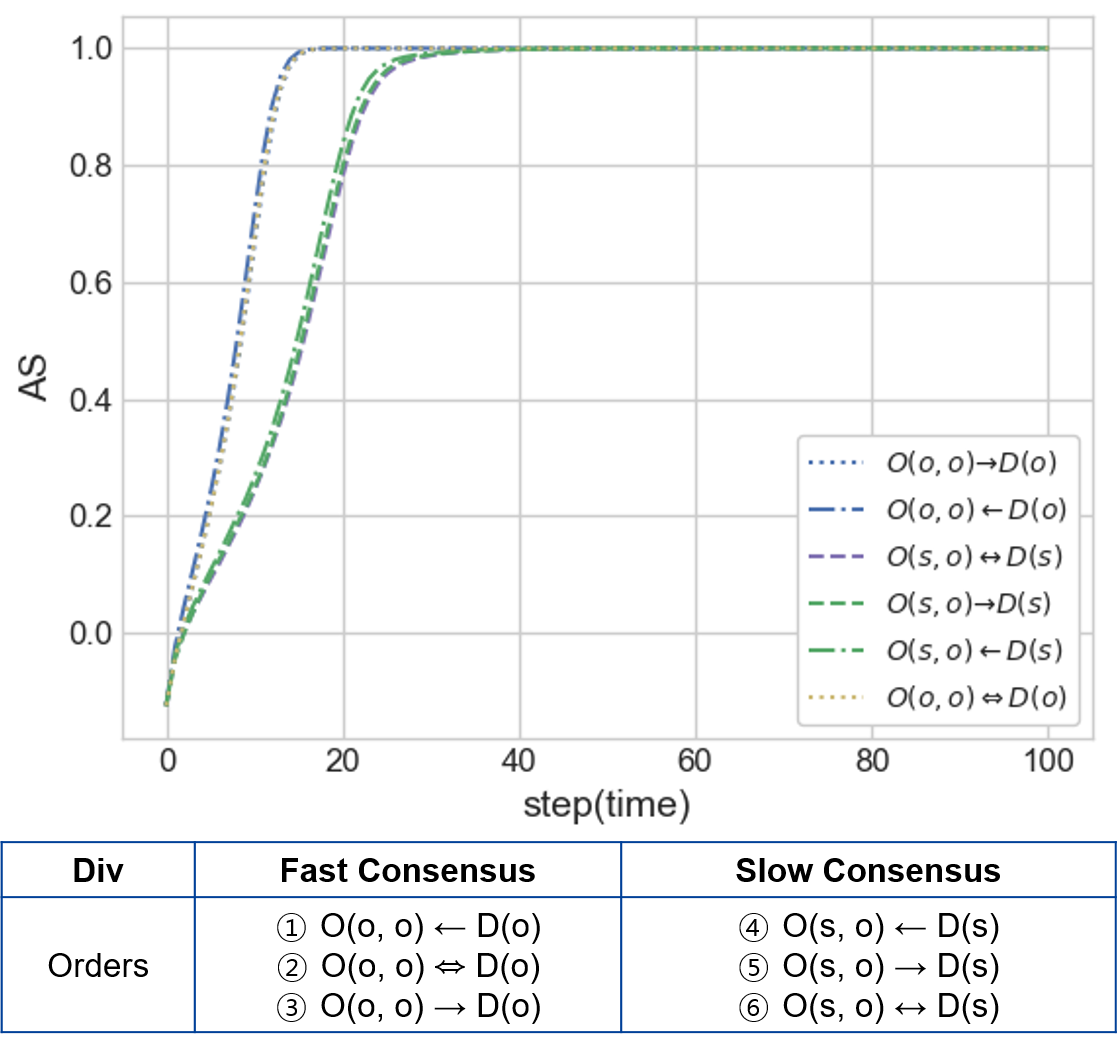
\includegraphics[width=\hsize]{chap4_layerorder.png}
	\caption{Simulation results according to orders of layers: Comparison between orders of layers under the same conditions such as orders of nodes and edges.}
	\label{chap4_layerorder}
\end{figure}

Fig.~\ref{chap4_layerorder} shows simulation results related to orders of layers. The graph line indicates \textit{AS} value per each step. If the line reaches to $1$ or $-1$, that means the state of network has a positive or negative consensus state.

As seen in Fig.~\ref{chap4_layerorder}, it is shown that there is little difference according to orders of layers, but there is difference according to order of nodes. Order of nodes would be described in next section. Consensus time and result are almost same, though dynamics order is different. Regardless of dynamics orders, when other conditions such as updating rules of nodes and edges, are same, the dynamics results are also very similar. It could be found out that dynamics order of layers does not have an significant influence on the network state. \\

\section{Order of nodes}
In the simulation model, each layer has $2048$ nodes, and each node has interactions with other nodes. Now, interaction order of nodes would be considered. One node can be updated sequentially after neighbor nodes are updated. Otherwise, every node can be updated simultaneously. And, nodes would be also updated randomly. As the method of random order, one edge is selected randomly and updated until all edges are considered regardless of nodes' orders or edges' orders.(For layer B, random order can not be applied because it has the formula that all edges of a node are considered together) Therefore, simulations would be implemented according to $3$ orders of nodes, such as sequential order, simultaneous order and random order. The interaction orders of nodes could be analyzed as communication methods in real world. If networks follow sequential updating rule of nodes, communication methods of networks might be translated as discussion or conversation with enough time. However, if networks follow simultaneous updating rules of nodes, communication methods of networks might be analyzed as vote or election.

\begin{figure}[!htb]
	\centering
	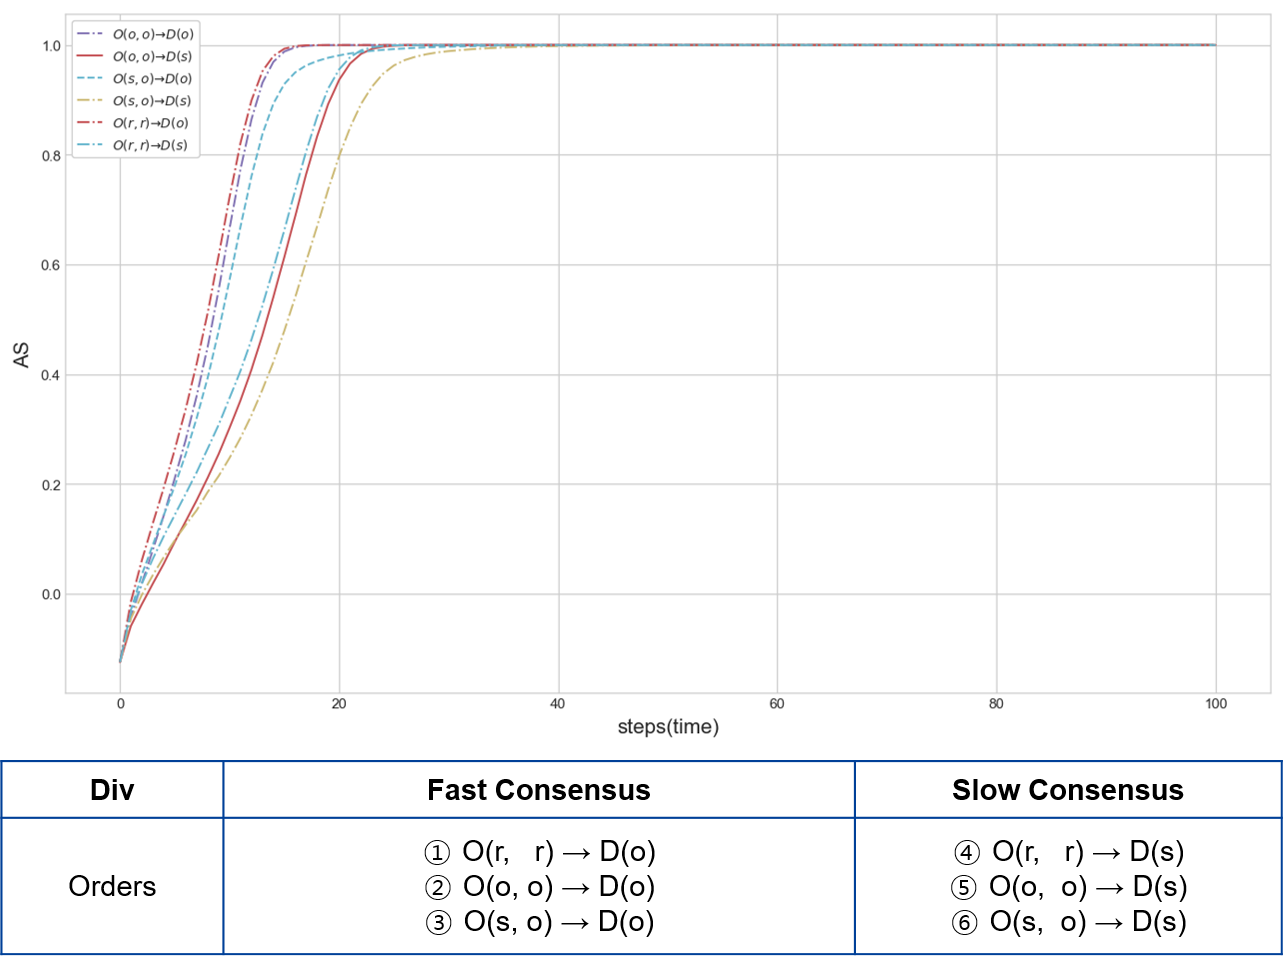
\includegraphics[width=\hsize]{figure/chap4_nodeorder.png}
	\caption{Simulation results according to orders of nodes: Comparison between orders of nodes under the same conditions such as orders of layers and edges.}
	\label{chap4_nodeorder}
\end{figure}

Fig.~\ref{chap4_nodeorder} shows simulation results according to interaction orders of nodes. The results are classified to two categories, fast consensus and slow consensus. It is shown that simultaneous interaction between nodes makes slow consensus. Simultaneous order in layer A does not make large difference with other orders in layer A, but it makes consensus slightly slow. Simultaneous interaction between nodes in layer B makes consensus slower than layer A. Random order has similar results with sequential order and does not make different states. 

To sum up, it is found out that simultaneous order of nodes makes slow consensus and sequential order of nodes makes fast consensus. In addition, interaction order of nodes in layer B has more influence on consensus time than in layer A. To make quick social consensus, both opinion layer and decision making layer would need sequential updating rule, such as conversation and discussion.\\     

\section{Order of edges}
Each node has several edges connected with other nodes. Updating rules can be divided according to that edges are activated sequentially or simultaneously. If edges of each node work sequentially, a state of node is changed whenever each edge is activated. However, If edges of a node are activated simultaneously, a state of node would be changed considering all connected nodes. In real world, order of edges in one node can be analyzed as characteristics of nodes. If order of edges is sequential, the node would be analyzed as rash because the state of node is changed whenever edges are activated. If order of edges is simultaneous, the node would be analyzed as considerate because it considers all connected nodes together. 

\begin{figure}[!htb]
	\centering
	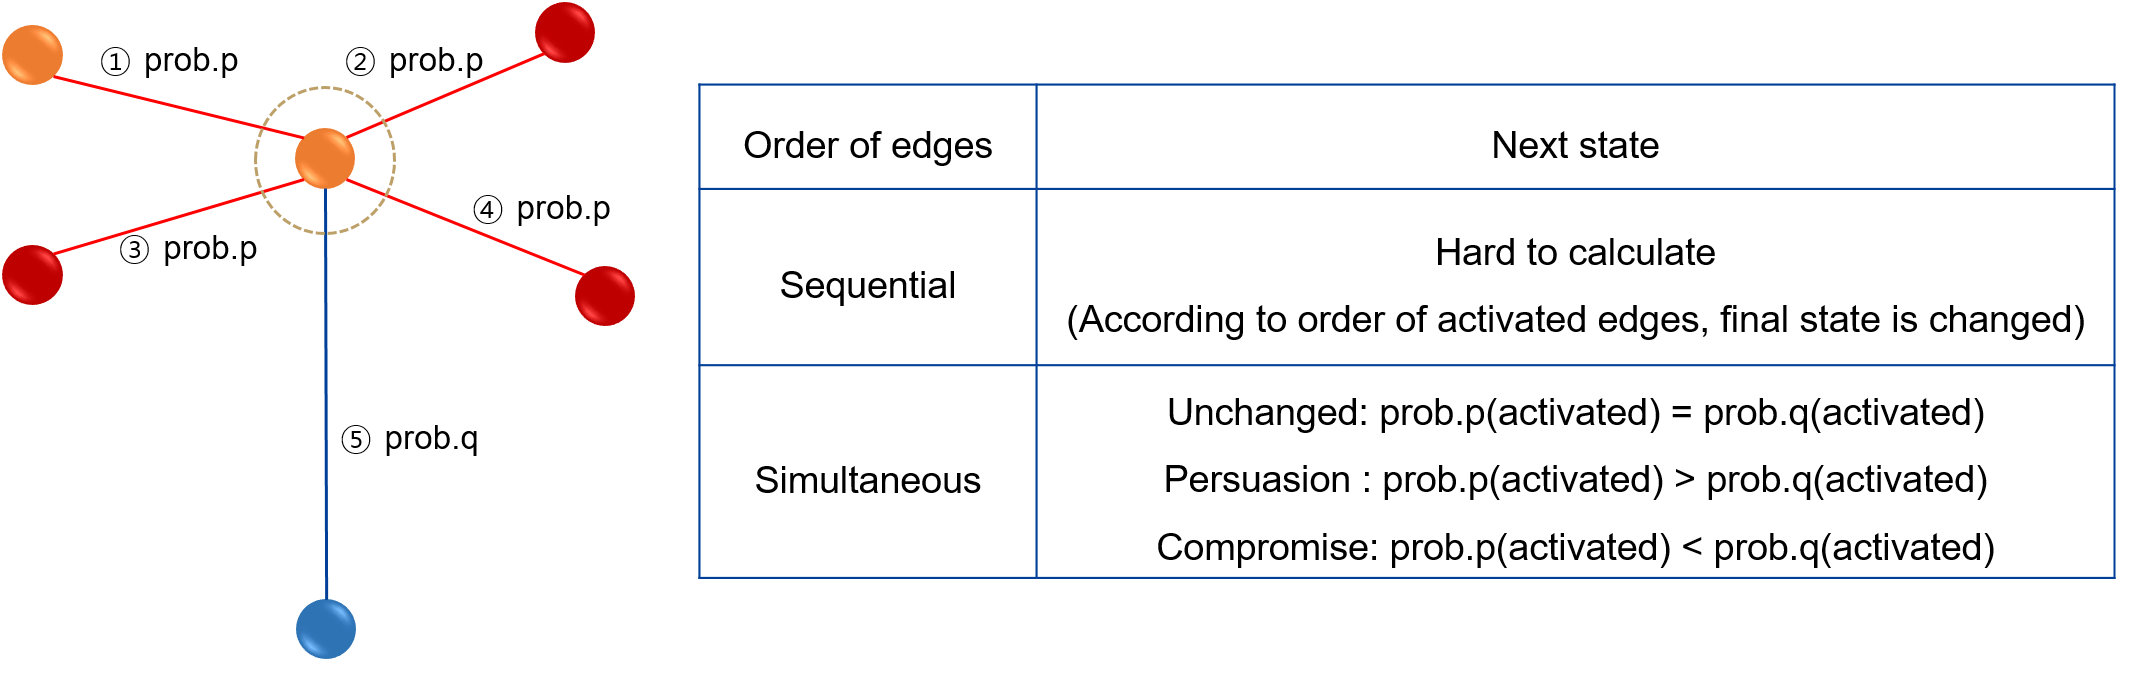
\includegraphics[width=\hsize]{figure/chap4_edgeorder_explanation.png}
	\caption{Order of edges: One node connected with other nodes is updated according to the sequential or simultaneous order of edges}
	\label{edgeorder_explanation}
\end{figure}  

For example, considering the case that one node is connected with other nodes as shown in Fig.~\ref{edgeorder_explanation}, we can think how the state of node changes according to edges' orders. If the edges follow the sequential updating rule, it is hard to calculate the probabilities because the state of node is continuously changed according to sequential edges' order. Therefore, the next states of nodes would be found by using computer simulation.

If the edges follow the simultaneous updating rule, it needs some assumptions as follows: 
\begin{enumerate}
	\item If the number of activated \textit{prob.p} is more than the number of activated \textit{prob.q}, persuasion dynamics would work. 
	\item If the number of activated \textit{prob.p} is same with the number of activated \textit{prob.q}, the state would be unchanged.
	\item If the number of activated \textit{prob.p} is less than the number of activated \textit{prob.q}, compromise dynamics would work.
\end{enumerate}

Through these assumptions, we can calculate probabilities of changing the state of node by considering all cases as these formula.  

\begin{equation}
\begin{array}{l}
K = \{ k \quad|\quad 0, \cdots ,{n^{ - {S_i}}}\}, \quad L = \{l \quad|\quad 0, \cdots ,{n^{{S_i}}}\},
\quad M = \{m \quad|\quad k-l\}, \\
{P_A}({S_i} \mapsto {{S'}_i}) = \begin{cases}
\mbox{unchanged}(k = l):\sum {{p^{{n^{ - {S_i}}}+m}} \cdot {{(1 - p)}^{{n^{{S_i}}}-m}} \cdot {}_{{n^{{S_{^i}}}}}{C_k} \cdot {}_{{n^{ - {S_{^i}}}}}{C_l}} \\
\mbox{compromise}(k > l):\sum {{p^{{n^{ - {S_i}}}+m}} \cdot {{(1 - p)}^{{n^{{S_i}}}-m}} \cdot {}_{{n^{{S_{^i}}}}}{C_k} \cdot {}_{{n^{ - {S_{^i}}}}}{C_l}} \\
\mbox{persuasion}(k < l):\sum {{p^{{n^{ - {S_i}}}+m}} \cdot {{(1 - p)}^{{n^{{S_i}}}-m}} \cdot {}_{{n^{{S_{^i}}}}}{C_k} \cdot {}_{{n^{ - {S_{^i}}}}}{C_l}} 
\end{cases}
\end{array}
\label{probabilities}
\end{equation}
In Eq.(\ref{probabilities}), $K$ means the set of integer from 0 to the number of nodes with the opposite state(${n^{ - {S_i}}}\}$). $L$ means the set of integer from 0 to the number of nodes with the same state(${n^{{S_i}}}\}$). By using permutations and combinations, these formula are derived.

\begin{figure}[!htb]
	\centering
	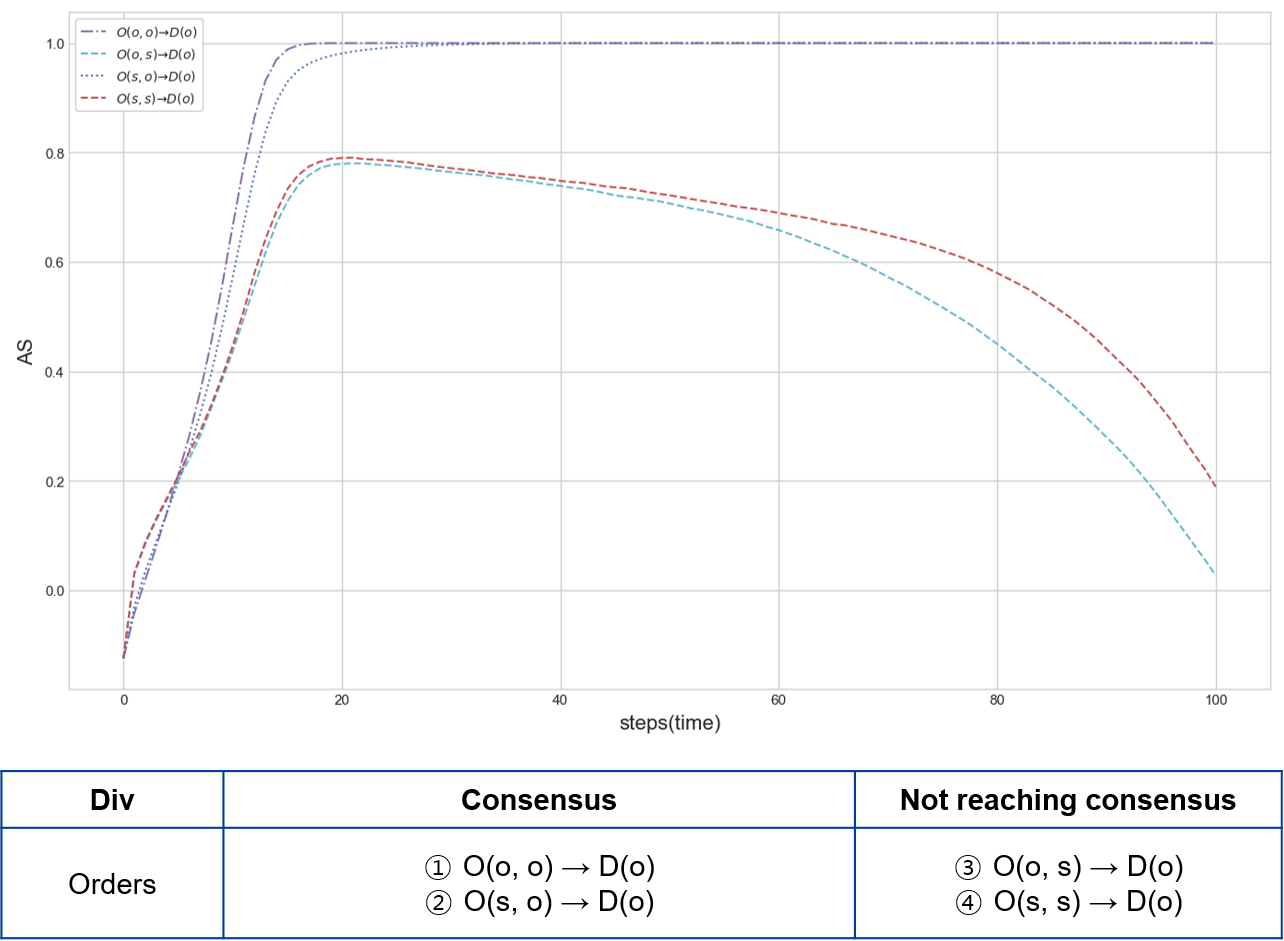
\includegraphics[width=\hsize]{figure/chap4_edgeorder.png}
	\caption{Simulation results according to orders of edges: Comparison between orders of edges under the same conditions such as orders of layers and nodes}
	\label{edgeorder}
\end{figure}

Fig.~\ref{edgeorder} shows the simulation result according to edges' orders. The results could be categorized to consensus and coexistence(not reaching consensus). Sequential updating rule of edges makes consensus under the same conditions such as orders of nodes and layers, i.e. rash nodes make consensus. But simultaneous updating rule of edges makes it hard to reach consensus under the same conditions such as orders of nodes and layers, i.e. considerate nodes do not make consensus. It can be analyzed that rash node is easy to be extreme and make consensus, but considerate node is very moderate and makes it hard to reach consensus.\\
 
\section{Comparison and Analysis}
It is found out that there are different simulation results according to orders of layers, nodes, and edges. To sum up all updating rules, they can be categorized into 3 parts, positive consensus, coexistence and negative consensus as shown in Fig.~\ref{ordertotal}.  
\begin{figure}[!htb]
	\centering
	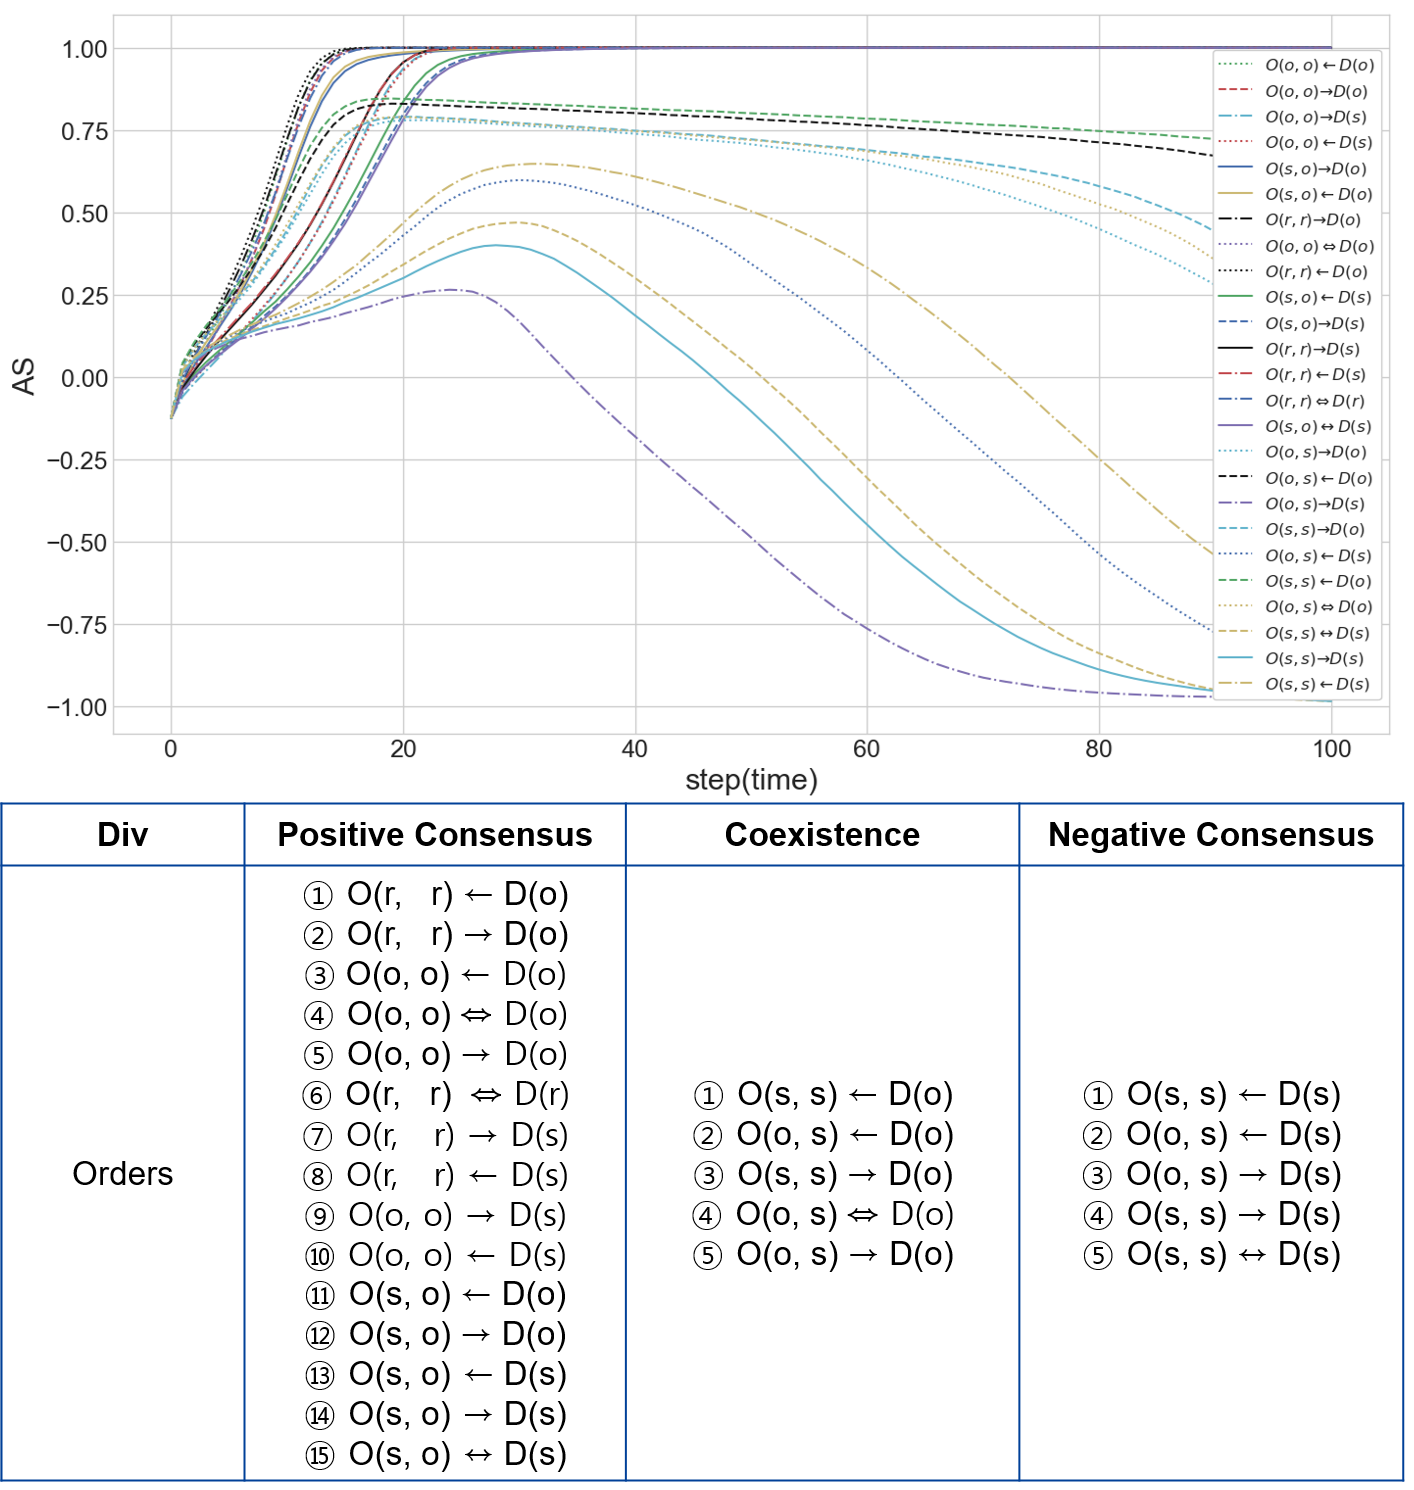
\includegraphics[width=\hsize]{figure/chap4_ordertotal.png}
	\caption{Total results of 25 updating rules with measuring \textit{AS}}
	\label{ordertotal}
\end{figure}

\begin{figure}[!htb]
	\centering
	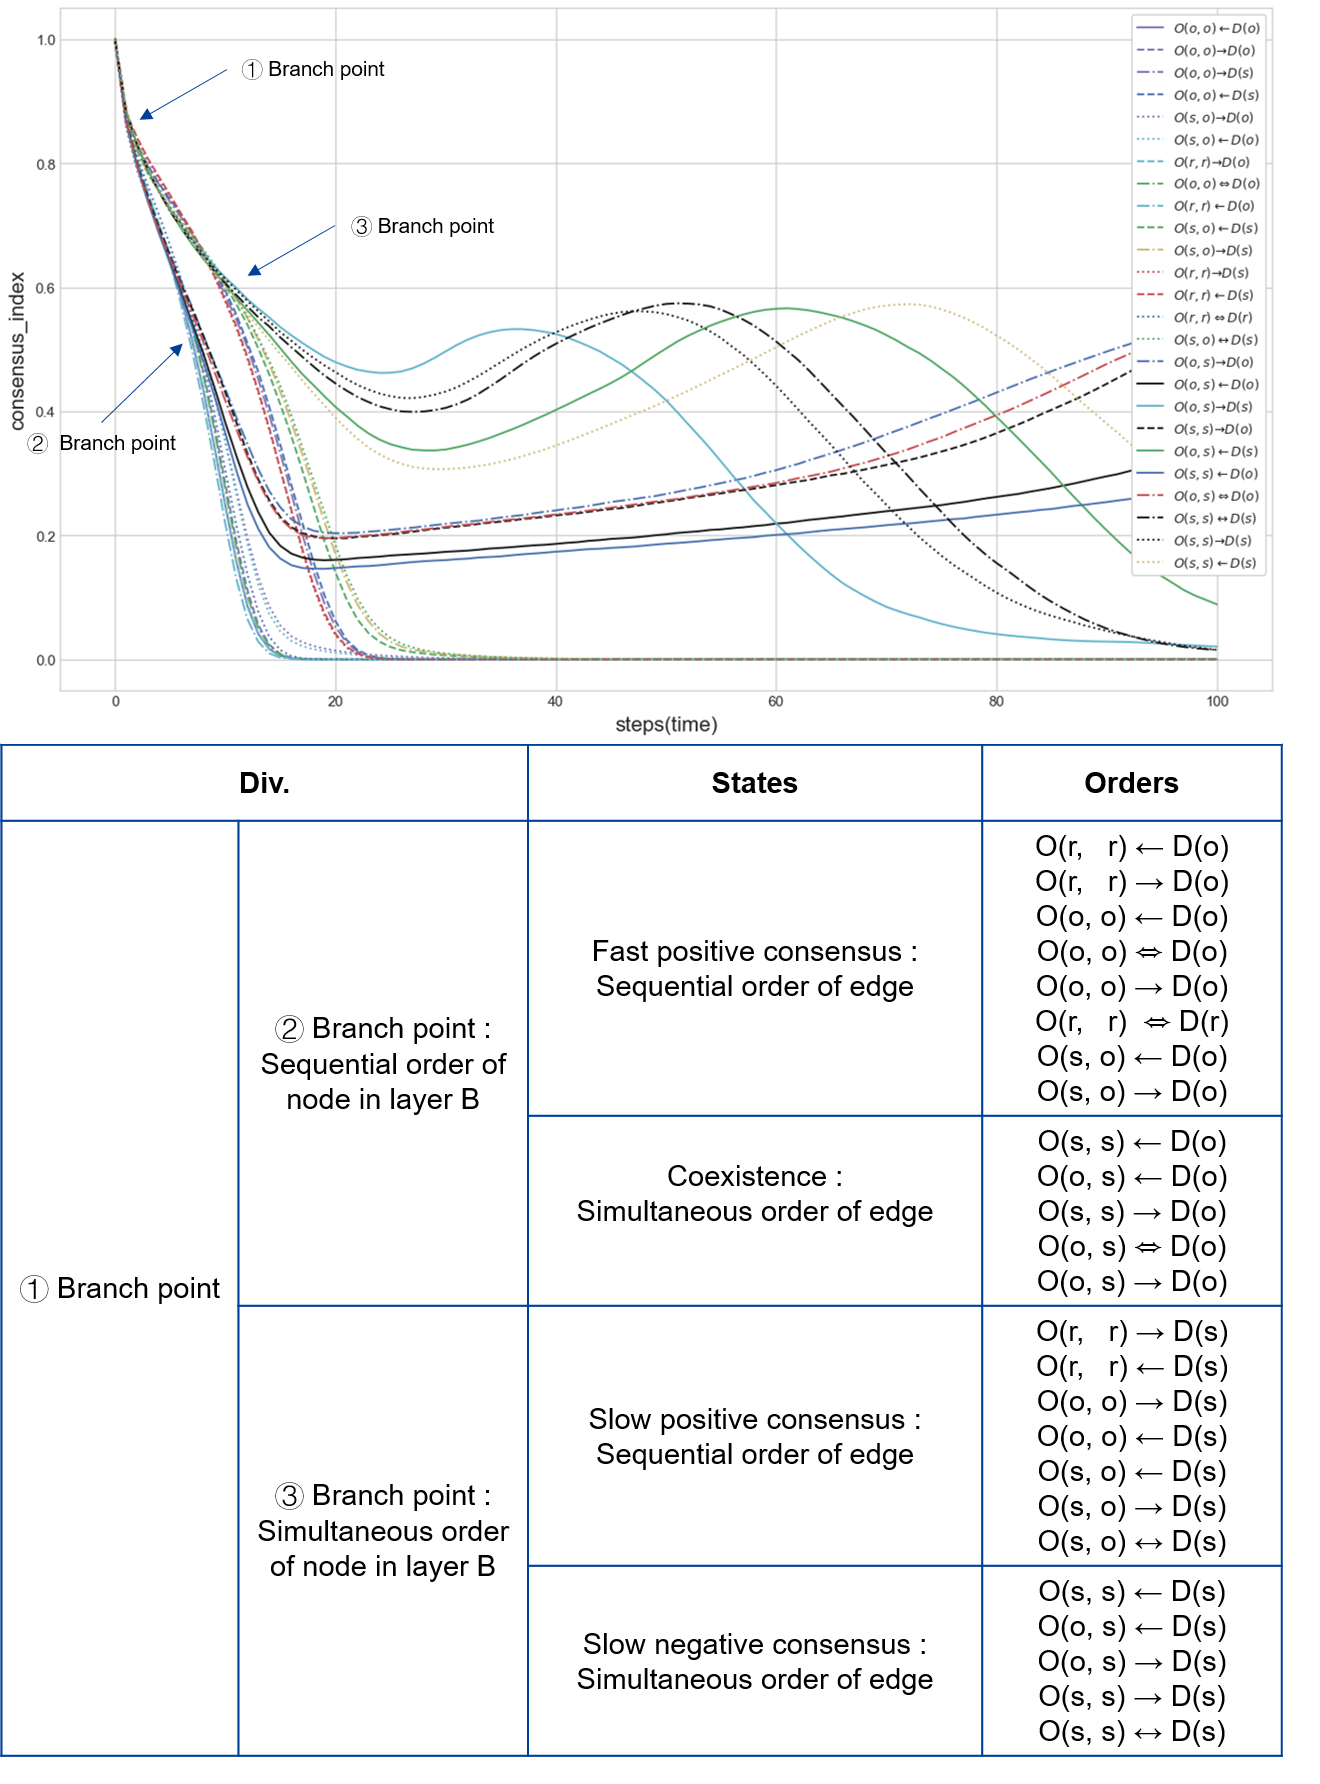
\includegraphics[width=\hsize]{figure/chap4_ordertotal2.png}
	\caption{Total results of 25 updating rules with measuring \textit{CI}}
	\label{ordertotal2}
\end{figure}

To clearly classify the state of two-layers, the results can be analyzed by using \textit{CI}, that measures how close the state of network is to consensus, as shown in Fig.~\ref{ordertotal2}. In this figure, there are three branch points. In the first branch point, the results are divided according to whether order of nodes in layer B is sequential or simultaneous. First branch point makes the results divided into fast convergent or slow convergent. In the second and third branch point, the results are divided according to whether order of edges in layer A is sequential or simultaneous. Second branch point makes the results divided into consensus or coexistence. Third branch point makes the results divided into positive consensus or negative consensus. To sum up, simulations results are classified into $4$ categories such as fast positive consensus, slow positive consensus, coexistence and slow negative consensus. The factors that make branch points have the vital influence for the state of networks. That means order of nodes(communication method) in layer B and order of edges(node characteristics) in layer A have very important role to make the state of network. It can be analyzed that communication method on decision-making layer makes fast or slow convergent for opinions and node characteristics on opinion layer makes the final state of networks such as positive consensus, negative consensus and coexistence. \\

\section{Conclusion}
Through these results, several important facts could be arranged. First, networks with simultaneous updating rules tend to make slow consensus or coexistence, sometimes make transition to opposite orientation. On the other hands, networks with sequential updating rules have a tendency to make fast consensus. Second, dynamics order between layers does not have an influence for network state, though there exists tiny consensus time gap. Third, order of nodes in layer B has more influence for network states than order of nodes in layer A because order of nodes in layer B makes the first branch point that has a vital role to make fast or slow convergent. That means the communication method in decision making layer is very important for determining consensus time. Fourth, order of edges in layer A is very influential so that it makes the second and third branch points that determine the final state of network. It can be analyzed as that characteristics of nodes in layer A, such as rash and considerate, has same orientation consensus or make transition to coexistence or opposite orientation consensus.



